\documentclass{article}
\usepackage{ketpic,ketlayer}
\usepackage{amsmath,amssymb}
\usepackage{graphicx}
\usepackage{xcolor}
\usepackage{bm,enumerate}
\usepackage[colorlinks=true,urlcolor=blue]{hyperref}

\setmargin{15}{15}{15}{15}

\renewcommand{\labelitemi}{$\cdot$}

\pagestyle{empty}

\begin{document}

\begin{center}
To Use KeTCindy 
\end{center}

\hfill Modified\ :\ \today

\begin{enumerate}[\bf\large 1.]\vspace{-1mm}
\item Install Cinderella, R, Maxima (and Sumatra only for Windows)\vspace{-1mm}
 \begin{itemize}
 \item \url{https://beta.cinderella.de}  (Cinderella)\\
\hspace*{6mm}Rem) In case of Windows, save first and right cliick to select 'Administrato'.\vspace{-1mm}
 \item \url{https://cran.r-project.org}   (R)\vspace{-1mm}
 \item \url{https://sourceforge.net/projects/maxima/files}  (Maxima)\vspace{-1mm}
 \item \url{https://www.sumatrapdfreader.org/download-free-pdf-viewer.html} (Sumatra)\\
\hspace*{5mm}Rem) Sumatra should be installed in Program Files (or x86).\vspace{-1mm}
 \end{itemize}
\item Install a TeX system if no one has been installed.\vspace{-1mm}
 \begin{enumerate}[(1)]
 \item TeXLive is recommended.\vspace{-1mm}
    \begin{itemize}
    \item KeTCindy has been implemented (2018 or later). Update first \verb|ketcindy|.\vspace{-1mm}
    \end{itemize}
 \item KeTTeX is a light-weighted TeXLive.\\
\hspace*{3mm}\url{https://github.com/ketpic/kettex/releases}\\
    \hspace*{6mm}Rem) See \verb|readmemore.pdf| in verb|doc>readmemore|,\vspace{-1mm}

\hspace*{3mm}\url{https://drive.google.com/drive/folders/1h_HDcKSp3S6qarbTSiUn9U5brgOGbU93?usp=sharing}\\
\hspace*{12mm}Mac (kettex.dmg)\hspace{3mm}Windows (kettex.exe)\hspace*{3mm}Linux (kettex.tar.xz)\\
\hspace*{3mm}Rem)Move unzipped kettex into the folder /Applications for Mac and C:\textbackslash\ for Windows.
 \end{enumerate}

\item Install KeTCindy as follows.\vspace{-1mm}
  \begin{enumerate}[(1)]
  \item Download ketcindy from CTAN(\url{https://ctan.org}).\\
  \hspace*{10mm}Search ketcindy $>$ Pack­age ketcindy $>$ Download\ \ ('ketcindy')\vspace{-1mm}
    \begin{itemize}
    \item[$\cdot$]The {\color{red}latest version} is downloadable from Repository:\\
         \hspace*{10mm}Code $>$ Download ZIP\ \ ('ketcindy-master')\\
        \hspace*{5mm}Rem) Case of Windows, move it to \verb|C:\|.\vspace{-1mm}
    \end{itemize}
  \item Double click \verb|ketcindysettings.cdy| in the folder.\vspace{-1mm}
    \begin{itemize}
    \item Set Cinderella as the executive program if necessary.\vspace{-1mm}
    \item Reboot Cinderella if other cdy files are open.\vspace{-1mm}
   \end{itemize}
  \item Select (1)(2) in the following figure, and execute (3) in the order left to right.
  \end{enumerate}

%\vspace{2mm}

\begin{layer}{140}{0}
\putnotese{17}{20}{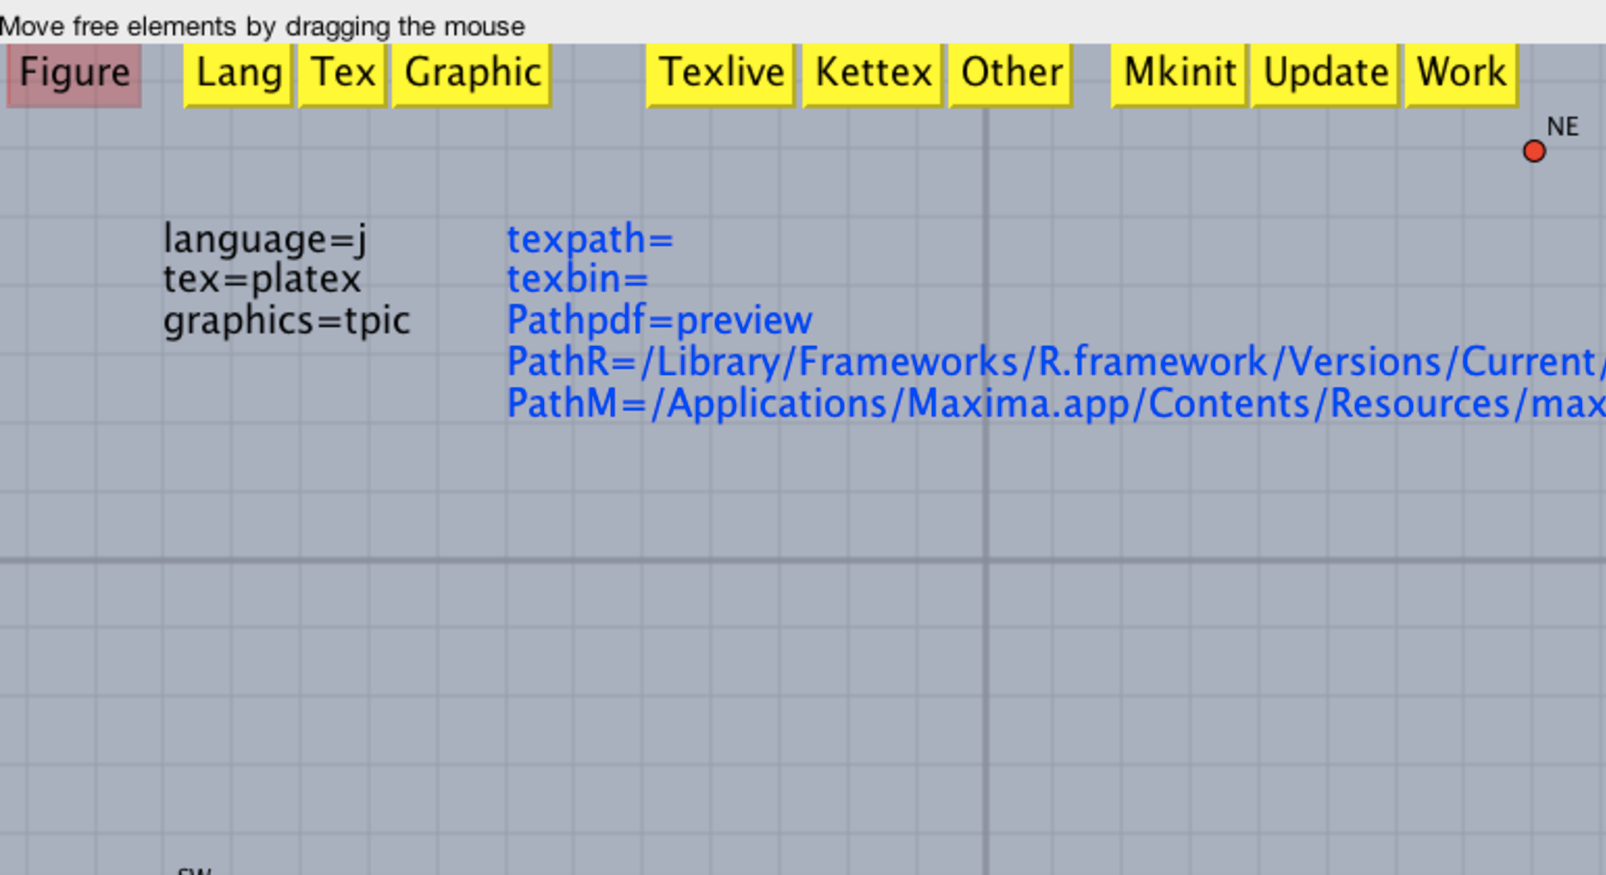
\includegraphics[bb=0.00 0.00 752.00 408.00,width=100mm]{Fig/setting.pdf}}
\putnotee{0}{5}{\bf [1]\ Select language,etc}
\putnotese{-7}{10}{\underline{Language}}
\putnotese{-5}{15}{\begin{tabular}{l}Japanese\\English\end{tabular}}
\putnotese{-7}{25}{\underline{\TeX}}
\putnotese{-5}{29}{\begin{tabular}{l}
platex\\uplatex\\latex\\xelatex\\pdflatex\\lualatex\end{tabular}}
\putnotese{-7}{56}{\underline{Graphic Code}}
\putnotese{-5}{60}{\begin{tabular}{l}tpic\\pict2e\\tikz\end{tabular}}
\arrowline{37}{20}{17}{135}
\putnoten{73}{7}{\bf [2]Select \TeX\ sytem}
\arrowline{73}{20}{13}{90}
\putnotee{115}{5}{\bf [3]\ Folder operation}
\arrowline{100}{20}{20}{45}
\putnotese{121}{10}{\fbox{Mkinit}}
\putnotese{123}{17}{\begin{minipage}[t]{52mm}%
Create initialization file in user's home(Home).\hfill Name: ketcindy.ini\\
%{\small Rm)\ If the file is moved into\\
%\hspace*{10mm} Cinderella/Plugins, \\
%\hspace*{1mm} Change CindyScript/ketlib to\\
%\hspace*{6mm} setdirectory(plugindirectory)}
\end{minipage}}
\putnotese{121}{30}{\fbox{Update}}
\putnotese{123}{37}{Update ketcindy in \TeX\ system}
%%\putnotese{126}{39}{Press Help for Run-time error}
\putnotese{121}{48}{\fbox{Work}}
\putnotese{123}{56}{\begin{minipage}[t]{52mm}%
Create folder 'ketcindy' in Home.\\
Manuals, samples will be copied.
\end{minipage}}
\end{layer}

\vspace{70mm}

\item Test run\vspace{-1mm}
\begin{itemize}
\item Quit once Cinderella and double click a file in the User's home\verb|/ketcindy/templtates|.\vspace{-1mm}
\item Press \verb|Figure| button, and the pdf will be displayed.\vspace{-1mm}
\end{itemize}

\item Others\vspace{-1mm}
\begin{itemize}
\item \verb|ketcindy.ini| will be generatede in the User's home as default.\\
\hspace*{5mm}$\cdot$\ Write \verb|setdirectory(gethome());| on the 3rd line in \verb|CindyScripts>ketlib|.\\
\hspace*{5mm}$\cdot$\ Write \verb|setdirectory(plugindirectory);| if \verb|ketincy.ini| is moved to Plugins in Cinderella.\vspace{-1mm}
\item See Readmemore for more informations.\vspace{-1mm}
\end{itemize}

  \end{enumerate}

\end{document}